% Options for packages loaded elsewhere
\PassOptionsToPackage{unicode}{hyperref}
\PassOptionsToPackage{hyphens}{url}
\PassOptionsToPackage{dvipsnames,svgnames,x11names}{xcolor}
%
\documentclass[
  a4paper,
]{article}
\usepackage{amsmath,amssymb}
\usepackage{iftex}
\ifPDFTeX
  \usepackage[T1]{fontenc}
  \usepackage[utf8]{inputenc}
  \usepackage{vntex} % Gói hỗ trợ tiếng Việt đầy đủ
  \usepackage{amsmath} % Hỗ trợ các ký hiệu Toán học
  \usepackage{textcomp} % provide euro and other symbols
\else % if luatex or xetex
  \usepackage{unicode-math} % this also loads fontspec
  \defaultfontfeatures{Scale=MatchLowercase}
  \defaultfontfeatures[\rmfamily]{Ligatures=TeX,Scale=1}
\fi
\usepackage{lmodern}
\ifPDFTeX\else
  % xetex/luatex font selection
\fi
% Use upquote if available, for straight quotes in verbatim environments
\IfFileExists{upquote.sty}{\usepackage{upquote}}{}
\IfFileExists{microtype.sty}{% use microtype if available
  \usepackage[]{microtype}
  \UseMicrotypeSet[protrusion]{basicmath} % disable protrusion for tt fonts
}{}
\makeatletter
\@ifundefined{KOMAClassName}{% if non-KOMA class
  \IfFileExists{parskip.sty}{%
    \usepackage{parskip}
  }{% else
    \setlength{\parindent}{0pt}
    \setlength{\parskip}{6pt plus 2pt minus 1pt}}
}{% if KOMA class
  \KOMAoptions{parskip=half}}
\makeatother
\usepackage{xcolor}
\usepackage[margin=1in]{geometry}
\usepackage{longtable,booktabs,array}
\usepackage{calc} % for calculating minipage widths
% Correct order of tables after \paragraph or \subparagraph
\usepackage{etoolbox}
\makeatletter
\patchcmd\longtable{\par}{\if@noskipsec\mbox{}\fi\par}{}{}
\makeatother
% Allow footnotes in longtable head/foot
\IfFileExists{footnotehyper.sty}{\usepackage{footnotehyper}}{\usepackage{footnote}}
\makesavenoteenv{longtable}
\usepackage{graphicx}
\makeatletter
\def\maxwidth{\ifdim\Gin@nat@width>\linewidth\linewidth\else\Gin@nat@width\fi}
\def\maxheight{\ifdim\Gin@nat@height>\textheight\textheight\else\Gin@nat@height\fi}
\makeatother
% Scale images if necessary, so that they will not overflow the page
% margins by default, and it is still possible to overwrite the defaults
% using explicit options in \includegraphics[width, height, ...]{}
\setkeys{Gin}{width=\maxwidth,height=\maxheight,keepaspectratio}
% Set default figure placement to htbp
\makeatletter
\def\fps@figure{htbp}
\makeatother
\setlength{\emergencystretch}{3em} % prevent overfull lines
\providecommand{\tightlist}{%
  \setlength{\itemsep}{0pt}\setlength{\parskip}{0pt}}
\setcounter{secnumdepth}{5}
\ifLuaTeX
\usepackage[bidi=basic]{babel}
\else
\usepackage[bidi=default]{babel}
\fi
\babelprovide[main,import]{vietnamese}
% get rid of language-specific shorthands (see #6817):
\let\LanguageShortHands\languageshorthands
\def\languageshorthands#1{}
\usepackage{setspace}
\usepackage{xcolor}
\usepackage{amsmath}
\usepackage{graphicx}
\usepackage{geometry}
\usepackage{hyperref}
\usepackage{fancyhdr}
\usepackage{setspace}
\onehalfspacing
\ifLuaTeX
  \usepackage{selnolig}  % disable illegal ligatures
\fi
\usepackage{bookmark}
\IfFileExists{xurl.sty}{\usepackage{xurl}}{} % add URL line breaks if available
\urlstyle{same}
\hypersetup{
  pdftitle={Đồ án -- Phân lớp},
  pdflang={vi},
  colorlinks=true,
  linkcolor={Maroon},
  filecolor={Maroon},
  citecolor={Blue},
  urlcolor={red},
  pdfcreator={LaTeX via pandoc}}

\title{Đồ án -- Phân lớp}
\usepackage{etoolbox}
\makeatletter
\providecommand{\subtitle}[1]{% add subtitle to \maketitle
  \apptocmd{\@title}{\par {\large #1 \par}}{}{}
}
\makeatother
\subtitle{Multivariate Statistical Applied}
\author{}
\date{\today}


\begin{document}
\maketitle
\begin{abstract}
Phân loại (Classification) là một trong những bài toán quan trọng trong
học máy (Machine Learning) và thống kê, với mục tiêu phân nhóm các đối
tượng dựa trên các đặc trưng (features) đã biết. Trong đó, Phân tích
phân biệt tuyến tính (Linear Discriminant Analysis - LDA) là một phương
pháp phổ biến, giúp tìm kiếm một không gian chiếu tối ưu để phân tách
các nhóm dữ liệu. LDA không chỉ giúp cải thiện khả năng phân loại mà còn
hỗ trợ giảm chiều dữ liệu, giúp tối ưu hóa hiệu suất tính toán và tránh
hiện tượng quá khớp (overfitting).

Trong bài toán phân loại hai lớp, LDA có thể được hiểu như Fisher's
Linear Discriminant (FLD), trong đó mục tiêu là tìm một vector chiếu tối
ưu để tối đa hóa độ phân biệt giữa hai lớp bằng cách tối đa hóa phương
sai giữa các lớp và tối thiểu hóa phương sai trong từng lớp. Tuy nhiên,
LDA không chỉ giới hạn trong bài toán hai lớp mà còn có thể mở rộng để
phân biệt nhiều lớp bằng cách tìm tập hợp các vector chiếu, giúp tối ưu
hóa khả năng phân tách giữa nhiều nhóm dữ liệu trong không gian đặc
trưng.

Trong nghiên cứu này, chúng tôi tiến hành thực nghiệm với một case study
thực tế, áp dụng LDA trên các tập dữ liệu có nhãn để đánh giá hiệu suất
của phương pháp này. Chúng tôi sử dụng các chỉ số đánh giá như độ chính
xác (Accuracy), độ nhạy (Sensitivity), độ đặc hiệu (Specificity) và
F1-score để đo lường khả năng phân loại của mô hình. Kết quả thực nghiệm
cho thấy rằng LDA hoạt động tốt khi dữ liệu có phân phối chuẩn và ma
trận hiệp phương sai đồng nhất giữa các lớp, nhưng có thể bị suy giảm
hiệu suất khi các giả định này không được thỏa mãn.

Bên cạnh đánh giá lý thuyết và thực nghiệm, chúng tôi cũng phân tích các
ứng dụng thực tế của LDA trong nhiều lĩnh vực khác nhau như nhận dạng
khuôn mặt, chẩn đoán y khoa, tài chính và sinh học. Với khả năng giảm
chiều dữ liệu hiệu quả trong khi vẫn bảo toàn thông tin quan trọng, LDA
trở thành một công cụ mạnh mẽ trong việc trích xuất đặc trưng và phân
loại dữ liệu có cấu trúc phức tạp.

Những phát hiện từ nghiên cứu này giúp cung cấp một cái nhìn toàn diện
về vai trò của LDA trong bài toán phân loại, từ bài toán phân biệt hai
lớp đơn giản đến bài toán phân biệt nhiều lớp, cùng với các ứng dụng
thực tế của nó.

Từ khóa: Phân loại (Classification), Phân tích phân biệt tuyến tính
(LDA), Fisher's Linear Discriminant (FLD), Học máy (Machine Learning),
Giảm chiều dữ liệu (Dimensionality Reduction), Ứng dụng LDA.
\end{abstract}

\pagebreak
\tableofcontents 
\pagebreak

\section{Giới thiệu}\label{giux1edbi-thiux1ec7u}

\subsection{Phân biệt (Discrimination) và Phân lớp
(Classification)}\label{phuxe2n-biux1ec7t-discrimination-vuxe0-phuxe2n-lux1edbp-classification}

\subsection{Ý nghĩa về khoa
học}\label{uxfd-nghux129a-vux1ec1-khoa-hux1ecdc}

\subsection{Ý nghĩa về ứng
dụng}\label{uxfd-nghux129a-vux1ec1-ux1ee9ng-dux1ee5ng}

\subsection{Phát biểu bài toán}\label{phuxe1t-biux1ec3u-buxe0i-touxe1n}

\begin{itemize}
\item
  \textbf{Giả sử:}

  \begin{itemize}
  \tightlist
  \item
    Có \(g\) nhóm khác nhau, ký hiệu \(G = \{G_1, G_2, \ldots, G_g\}\).
    Mỗi nhóm có một phân phối xác suất riêng với trung bình \(\mu_G\) và
    ma trận hiệp phương sai \(\Sigma_G\).
  \item
    Một quan sát \(x\) có \(d\) đặc trưng và thuộc về một trong các nhóm
    \(G\).
  \end{itemize}
\item
  \textbf{Đầu vào:}

  \begin{itemize}
  \tightlist
  \item
    Tập dữ liệu gồm \(n\) mẫu, mỗi mẫu có \(d\) đặc trưng:
    \[X = \{x_1, x_2, \ldots, x_n\}, \quad x_i \in \mathbb{R}^d\]
  \item
    Nhãn tương ứng với các mẫu:
    \[Y = \{y_1, y_2, \ldots, y_n\}, \quad y_i \in \{G_1, G_2, \ldots, G_g\}\]
  \end{itemize}
\item
  \textbf{Đầu ra:} Nhóm \(G^*\) tối ưu cho một quan sát mới \(x\), xác
  định theo: \[G^* = \arg\max_{G} P(G | x)\] hoặc theo hàm phân biệt
  (discriminant function): \[G^* = \arg\max_{G} \delta_G(x)\]
\item
  \textbf{Mục tiêu của bài toán:} là xây dựng một hàm phân loại \(f\) để
  gán một quan sát \(x\) có \(d\) đặc trưng vào một trong \(g\) nhóm
  (classes) sao cho tối ưu được độ chính xác phân loại.

  Cụ thể, cần tìm một ánh xạ:
  \[f: \mathbb{R}^d \to \{G_1, G_2, \ldots, G_g\}\] sao cho với mỗi quan
  sát \(x\), nhóm dự đoán \(G^* = f(x)\) là nhóm có xác suất hậu nghiệm
  cao nhất hoặc hàm phân biệt tối đa.
\end{itemize}

\subsubsection{Cấu trúc chung
(Framework)}\label{cux1ea5u-truxfac-chung-framework}

\begin{figure}
\centering
\includegraphics[width=0.5\textwidth,height=\textheight]{}
\caption{Mô hình cấu trúc chung của bài toán phân lớp}
\end{figure}

\subsubsection{Đóng góp}\label{ux111uxf3ng-guxf3p}

Một câu hỏi quan trọng là làm thế nào để xác định hàm phân biệt
(\(\delta_G(x)\)). Một trong những phương pháp phổ biến để giải quyết
vấn đề này là Phân tích Phân biệt Tuyến tính (LDA). Tương tự như Phân
tích Thành phần Chính (PCA), LDA chiếu toàn bộ tập dữ liệu lên một siêu
phẳng có số chiều nhỏ hơn, với mục tiêu phân tách dữ liệu một cách rõ
ràng hơn. Hàm phân biệt \(\delta_G(x)\) trong LDA có dạng tuyến tính,
cho phép phân tách các lớp bằng cách tìm ra hướng chiếu tối ưu nhất.

Vì thế, nghiên cứu này đóng góp vào lĩnh vực phân loại dữ liệu bằng cách
cung cấp một đánh giá toàn diện về Phân tích Phân biệt Tuyến tính (LDA)
từ cả góc độ lý thuyết và thực nghiệm. Cụ thể, các đóng góp chính của
nghiên cứu bao gồm:

\begin{enumerate}
\def\labelenumi{\arabic{enumi}.}
\item
  \textbf{Phân tch chi tiết về LDA trong bài toán phân loại:}

  Nghiên cứu trình bày một cách hệ thống nguyên lý hoạt động của LDA,
  bao gồm cách tiếp cận Fisher's Linear Discriminant (FLD) trong bài
  toán phân loại hai lớp và cách mở rộng phương pháp này cho nhiều lớp
  dữ liệu. Chúng tôi thảo luận các giả định quan trọng của LDA, bao gồm
  tính phân phối chuẩn của dữ liệu và tính đồng nhất của ma trận hiệp
  phương sai giữa các lớp.
\item
  \textbf{Đánh giá thực nghiệm hiệu suất của LDA:}

  Chúng tôi thực hiện các thí nghiệm trên các tập dữ liệu có nhãn để
  đánh giá hiệu suất phân loại của LDA trong các điều kiện khác nhau.
  Các chỉ số đánh giá như \ldots.. được sử dụng để định lượng hiệu quả
  của mô hình. Kết quả thực nghiệm cho thấy LDA có hiệu suất tốt khi dữ
  liệu tuân theo các giả định lý thuyết, nhưng có thể bị suy giảm khi vi
  phạm các giả định này.
\item
  \textbf{Phân tích ứng dụng thực tế của LDA:}

  Nghiên cứu và áp dụng ứng dụng thực tế của LDA trên tập dữ liệu tiêu
  chuẩn để đánh giá tính ứng dụng và hiệu suất của phương pháp này.
  Chúng tôi nhấn mạnh vai trò của LDA trong việc trích xuất đặc trưng và
  giảm chiều dữ liệu, đặc biệt trong các bài toán có số lượng đặc trưng
  lớn và yêu cầu tối ưu hóa tính toán.
\end{enumerate}

\pagebreak

\section{Các công trình nghiên cứu liên
quan}\label{cuxe1c-cuxf4ng-truxecnh-nghiuxean-cux1ee9u-liuxean-quan}

\subsection{Phân tích phân biệt tuyến tính (Linear Discriminant
Analysis)}\label{phuxe2n-tuxedch-phuxe2n-biux1ec7t-tuyux1ebfn-tuxednh-linear-discriminant-analysis}
\subsubsection{Phát biểu bài toán LDA tổng quát}  

Cho tập dữ liệu gồm \( N \) điểm \( \mathbf{x}_1, \mathbf{x}_2, ..., \mathbf{x}_N \) trong không gian \( d \)-chiều.  
Các điểm dữ liệu được chia thành \( K \) lớp, với mỗi lớp \( k \) chứa \( N_k \) điểm.  
Ký hiệu tập chỉ số của lớp \( k \) là:  
\[
\mathbf{C}_k = \{ n \; | \; n \in \text{lớp } k \}, \quad k = 1,2,...,K.
\]  
\textbf{Đầu ra}  

Ma trận chiếu \( W \in \mathbb{R}^{d \times (K-1)} \), trong đó mỗi cột là một vector chiếu \( \mathbf{w}_i \).  
Dữ liệu sau khi chiếu xuống không gian mới:  
\[
\mathbf{y}_n = W^T \mathbf{x}_n, \quad 1 \leq n \leq N.
\]  
Với \( \mathbf{y}_n \) thuộc không gian \( (K-1) \)-chiều  sao cho các điểm dữ liệu thuộc các lớp khác nhau được phân tách tốt nhất trong không gian mới này.

 
\subsubsection{Ý tưởng giải quyết bài toán}  

Để tiếp cận bài toán phân lớp nhiều lớp, trước hết xem xét bài toán đơn giản nhất: phân loại hai lớp.  

\textbf{Bài toán LDA hai lớp}  

Xét bài toán phân loại hai lớp (lớp \( C_1 \) - màu đỏ và lớp \( C_2 \) - màu xanh).  

\begin{figure}[htbp]
    \centering
    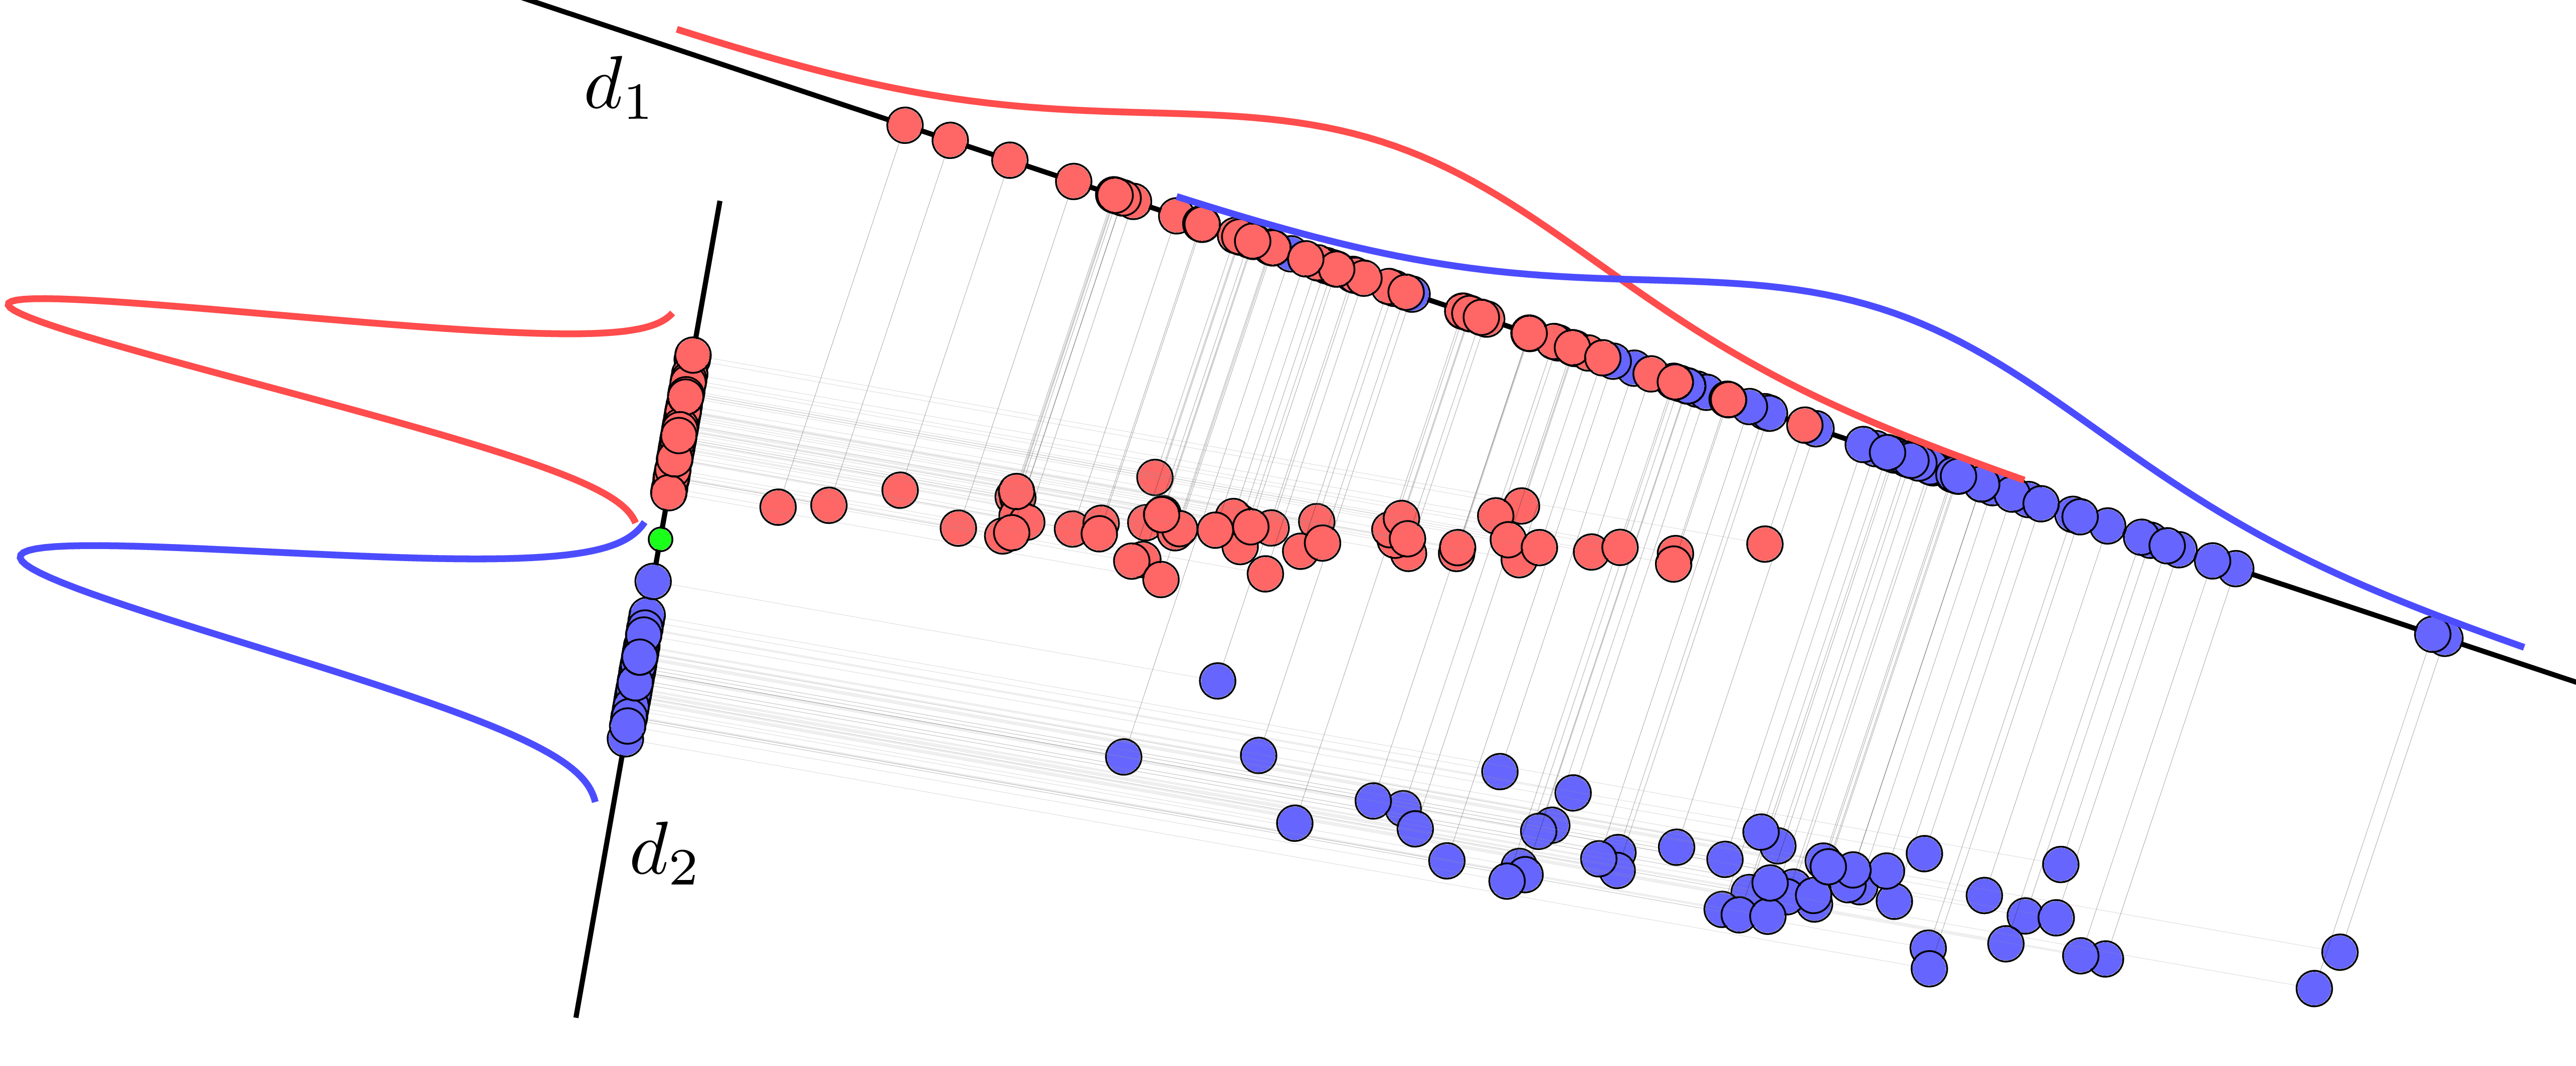
\includegraphics[width=0.6\textwidth]{assets/2_1_1.png}
    \caption{Trực quan hóa dữ liệu }
    \label{fig:example}
\end{figure}
  
\textbf{Giả sử:}  
\begin{itemize}
    \item Dữ liệu của hai lớp có phân phối chuẩn.  
    \item Giá trị kỳ vọng của mỗi lớp lần lượt là \( \mathbf{m}_1 \) và \( \mathbf{m}_2 \). 
    \item Độ phân tán của dữ liệu trong từng lớp được đo bằng phương sai \( s_1^2 \) và \( s_2^2 \).
\end{itemize}

\textbf{Bài toán đưa về thành:} Tìm một hướng chiếu \( \mathbf{w} \) sao cho dữ liệu của hai lớp tách biệt rõ ràng nhất.

Trước khi tìm lời giải, ta xét các trường hợp về cách dữ liệu bị phân tán khi chiếu lên một trục bất kỳ.  

\hspace{1cm}\textbf{Trường hợp 1: Hai lớp dữ liệu có phương sai lớn}  

\begin{figure}[htbp]
    \centering
    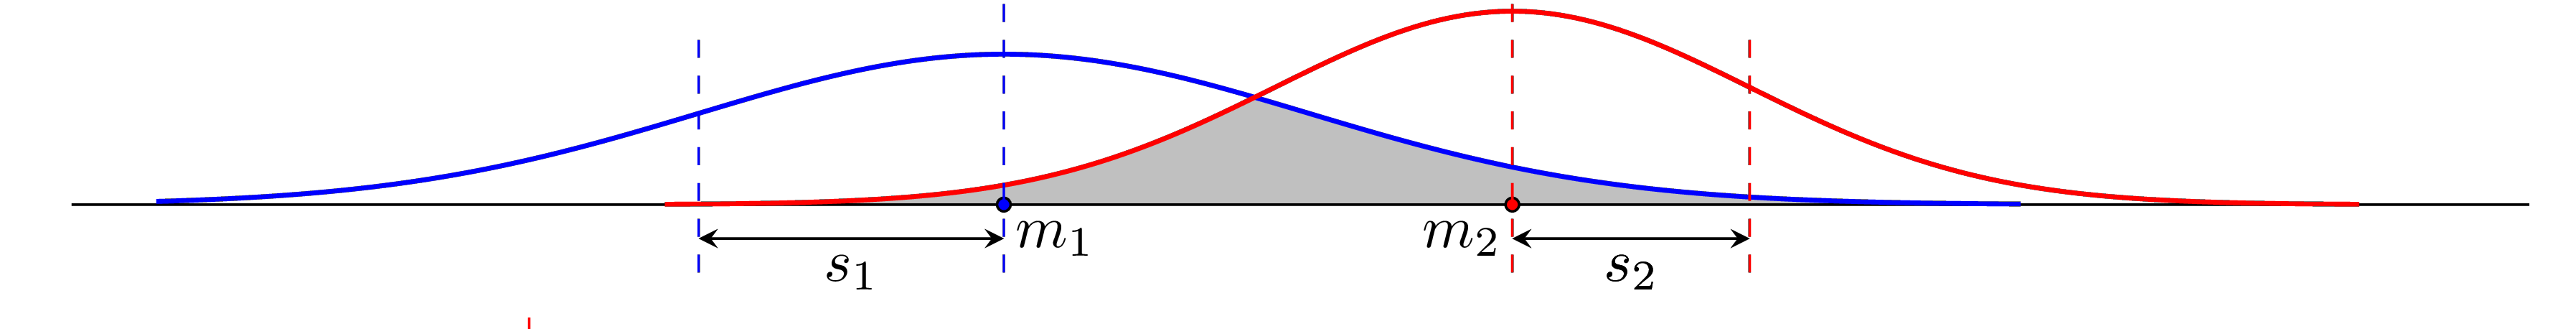
\includegraphics[width=0.9\textwidth]{assets/2_1_1a.png}
    \caption{Trường hợp 1: Phương sai lớn làm dữ liệu chồng lấn nhiều}
    \label{fig:case1}
\end{figure}

\hspace{1cm}Khi dữ liệu trong mỗi lớp có phương sai lớn, các điểm dữ liệu bị trải rộng và có phần chồng lấn lớn.  

\hspace{1cm}\textbf{Trường hợp 2: Phương sai nhỏ nhưng khoảng cách giữa trung tâm hai lớp quá gần}  

\begin{figure}[htbp]
    \centering
    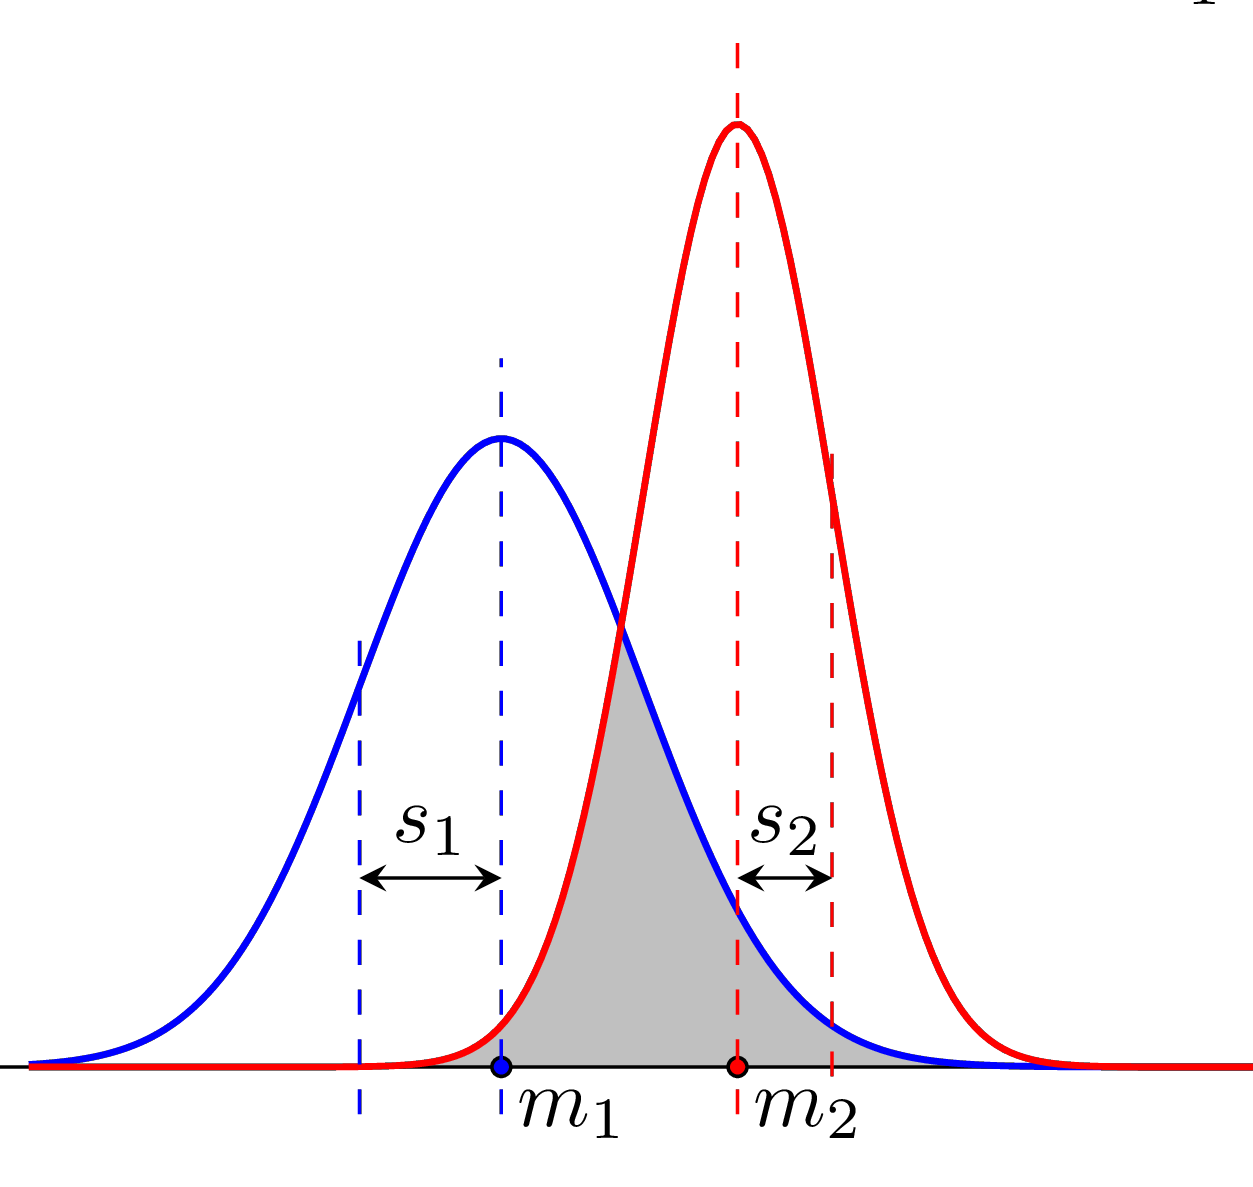
\includegraphics[width=0.3\textwidth]{assets/2_1_1b.png}
    \caption{Trường hợp 2: Trung tâm hai lớp quá gần nhau}
    \label{fig:case2}
\end{figure}

\hspace{1cm}Khi phương sai nhỏ, dữ liệu trong từng lớp ít phân tán, nhưng nếu trung tâm hai lớp \( \mathbf{m}_1 \) và \( \mathbf{m}_2 \) gần nhau, phần chồng lấn giữa hai lớp vẫn lớn.  

\hspace{1cm}\textbf{Trường hợp 3: Phương sai nhỏ và khoảng cách giữa hai trung tâm đủ lớn}  

\begin{figure}[htbp]
    \centering
    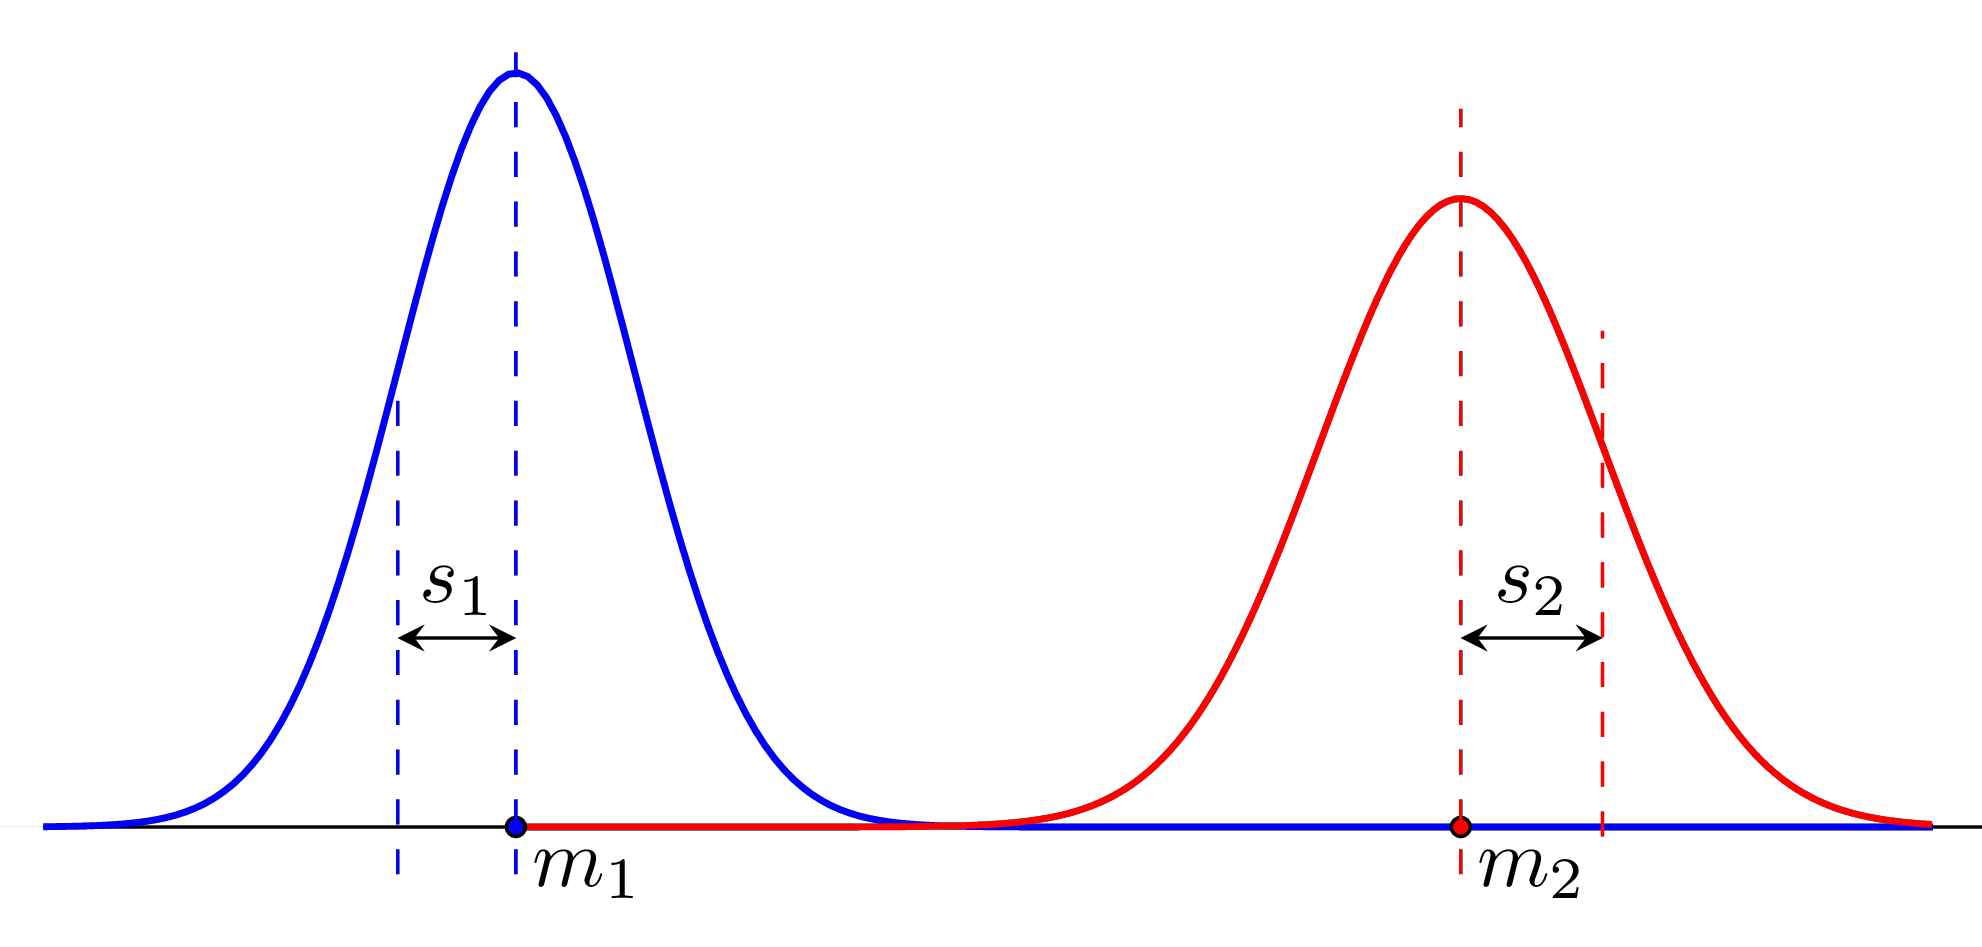
\includegraphics[width=0.5\textwidth]{assets/2_1_1c.png}
    \caption{Trường hợp 3: Phân bố tốt nhất để phân lớp}
    \label{fig:case3}
\end{figure}

\hspace{1cm}Khi dữ liệu trong mỗi lớp tập trung (phương sai nhỏ) và hai trung tâm cách xa nhau, phần chồng lấn giữa hai lớp được giảm đáng kể.  

\textbf{Ý tưởng bài toán LDA}  

Từ ba trường hợp trên, để có một hướng chiếu tối ưu cho phân loại, ta cần:  
\begin{itemize}
    \item Giảm phương sai trong mỗi lớp, giúp dữ liệu của từng lớp ít phân tán hơn.  
    \item Tăng khoảng cách giữa trung tâm hai lớp, giúp hai lớp cách xa nhau hơn, giảm phần chồng lấn.  
\end{itemize}

\textbf{Tổng quát hóa lên bài toán nhiều lớp}  

\hspace{1cm}Khi mở rộng lên bài toán với \( K \) lớp, ý tưởng vẫn giữ nguyên: tìm một không gian chiếu sao cho tỉ số giữa phương sai giữa các lớp và phương sai trong từng lớp là lớn nhất.  
Thay vì chỉ dùng một vector chiếu \( \mathbf{w} \) như bài toán hai lớp, LDA tổng quát sử dụng ma trận chiếu \( W \) với \( K-1 \) hướng chiếu tối ưu.  
Toán học đằng sau việc tìm các hướng chiếu này dựa trên việc tối ưu hóa tỉ số giữa ma trận tán sắc giữa các lớp \( S_B \) và ma trận tán sắc trong lớp \( S_W \).  
Việc tìm nghiệm của bài toán tương đương với việc tính các vector riêng của ma trận \( S_W^{-1} S_B \).  


\subsection{Phân biệt cực đại hợp lý (Maximum Likelihood
Discriminant)}\label{phuxe2n-biux1ec7t-cux1ef1c-ux111ux1ea1i-hux1ee3p-luxfd-maximum-likelihood-discriminant}
\subsubsection{Giới thiệu}
 
Phân biệt cực đại hợp lý (Maximum Likelihood Discrimination - MLD) là một phương pháp phân loại dựa trên nguyên lý xác suất. Ý tưởng chính là ước lượng xác suất để một điểm dữ liệu thuộc về một lớp cụ thể, sau đó gán nhãn cho điểm đó theo lớp có xác suất lớn nhất.  

\subsubsection{Cơ sở toán học}
Phương pháp này dựa trên các khái niệm xác suất và thống kê, đặc biệt là xác suất tiên nghiệm, xác suất có điều kiện và ước lượng tham số theo nguyên lý hợp lý cực đại (MLE). Để hiểu rõ hơn, trước tiên ta cần xây dựng nền tảng toán học quan trọng.

\textbf{Xác suất tiên nghiệm và xác suất có điều kiện}  \\
Mỗi lớp dữ liệu $C_k$ có một xác suất tiên nghiệm $P(C_k)$, phản ánh tỷ lệ xuất hiện của lớp đó trong tổng thể dữ liệu. Để xác định lớp của một điểm dữ liệu, ta cần xét xác suất có điều kiện $P(\mathbf{x} | C_k)$. Theo định lý Bayes:
\begin{equation}\tag{2.2.1}
P(C_k | \mathbf{x}) = \frac{P(\mathbf{x} | C_k) P(C_k)}{P(\mathbf{x})}
\end{equation}

với $P(\mathbf{x})$ là xác suất quan sát dữ liệu:
\begin{equation}\tag{2.2.2}
P(\mathbf{x}) = \sum_{j} P(\mathbf{x} | C_j) P(C_j)
\end{equation}

Để quyết định một điểm thuộc về lớp nào, ta chỉ cần so sánh giá trị xác suất hậu nghiệm \( P(C_k | \mathbf{x}) \) cho từng lớp và chọn lớp có xác suất lớn nhất. LDA dựa trên giả định rằng xác suất có điều kiện \( P(\mathbf{x} | C_k) \) tuân theo phân phối chuẩn, giúp đơn giản hóa mô hình và xác định được tiêu chí phân tách tối ưu.

\textbf{Hàm mật độ xác suất}  \\
Với giả định là dữ liệu trong mỗi lớp tuân theo phân phối chuẩn (Gaussian):
\begin{equation}\tag{2.2.3}
P(\mathbf{x} | C_k) = \frac{1}{(2\pi)^{d/2} |\Sigma_k|^{1/2}} \exp\left( -\frac{1}{2} (\mathbf{x} - \mu_k)^T \Sigma_k^{-1} (\mathbf{x} - \mu_k) \right)
\end{equation}
trong đó $\mu_k$ là vector trung bình và $\Sigma_k$ là ma trận hiệp phương sai.

Giả định phân phối chuẩn giúp đơn giản hóa bài toán phân loại vì nó cho phép ta mô hình hóa dữ liệu theo một mô hình toán học rõ ràng. Nếu các lớp dữ liệu thực sự tuân theo phân phối chuẩn với cùng một ma trận hiệp phương sai, thì ranh giới phân loại sẽ là một đường thẳng hoặc mặt phẳng (trong không gian nhiều chiều). Điều này giải thích vì sao LDA là một bộ phân loại tuyến tính.

\textbf{Ước lượng hợp lý cực đại (Maximum Likelihood Estimation - MLE)}  \\  
Trong bài toán phân loại, ta cần ước lượng các tham số của phân phối xác suất \( P(\mathbf{x} | C_k) \) để có thể tính được xác suất hậu nghiệm \( P(C_k | \mathbf{x}) \). Một trong những phương pháp phổ biến nhất để ước lượng tham số là phương pháp hợp lý cực đại (MLE), nhằm tìm các giá trị tham số tối ưu sao cho xác suất quan sát dữ liệu là lớn nhất.

Giả sử dữ liệu trong mỗi lớp \( C_k \) tuân theo phân phối chuẩn \( \mathcal{N}(\mu_k, \Sigma_k) \), ta thực hiện \textbf{Ước lượng tham số của phân phối chuẩn}  

Cho tập dữ liệu \( X = \{ x_1, x_2, ..., x_n \} \) được lấy mẫu từ một phân phối chuẩn một chiều \( \mathcal{N}(\mu, \sigma^2) \), ta cần tìm giá trị ước lượng của các tham số \( \mu \) (trung bình) và \( \sigma \) (độ lệch chuẩn).  

Hàm mật độ xác suất (PDF) của một điểm dữ liệu là:

\begin{equation}
f(x | \mu, \sigma) = \frac{1}{\sqrt{2\pi\sigma^2}} e^{-\frac{(x - \mu)^2}{2\sigma^2}}
\tag{2.2.4}
\end{equation}


Khi có nhiều quan sát độc lập \( X = \{x_1, x_2, \dots, x_n\} \), hàm hợp lý là tích các xác suất của từng điểm dữ liệu:

\begin{equation}
L(\mu, \sigma | X) = \prod_{i=1}^{n} f(x_i | \mu, \sigma)
\tag{2.2.5}
\end{equation}


Thay biểu thức \( f(x | \mu, \sigma) \) vào, ta có:

\begin{equation}
L(\mu, \sigma | X) = \prod_{i=1}^{n} \frac{1}{\sqrt{2\pi\sigma^2}} e^{-\frac{(x_i - \mu)^2}{2\sigma^2}}
\tag{2.2.6}
\end{equation}

Vì việc làm việc với tích nhiều số mũ có thể phức tạp, ta thường lấy log của hàm hợp lý (log-likelihood):

\[
\log L(\mu, \sigma | X) = \sum_{i=1}^{n} \log \left( \frac{1}{\sqrt{2\pi\sigma^2}} e^{-\frac{(x_i - \mu)^2}{2\sigma^2}} \right)
\]

\begin{equation}
= -\frac{n}{2} \log(2\pi) - n \log(\sigma) - \frac{1}{2\sigma^2} \sum_{i=1}^{n} (x_i - \mu)^2
\tag{2.2.7}
\end{equation}

\textit{Tìm ước lượng MLE cho \( \mu \)}  

Lấy đạo hàm của log-likelihood theo \( \mu \):

\[
\frac{\partial \log L}{\partial \mu} = \frac{1}{\sigma^2} \sum_{i=1}^{n} (x_i - \mu)
\]

Đặt bằng 0 để tìm giá trị cực đại:

\[
\sum_{i=1}^{n} (x_i - \mu) = 0
\]

Suy ra:

\begin{equation}
\mu_{MLE} = \frac{1}{n} \sum_{i=1}^{n} x_i
\tag{2.2.8}
\end{equation}

Như vậy, giá trị ước lượng hợp lý cực đại của \( \mu \) chính là trung bình mẫu.

\textit{Tìm ước lượng MLE cho \( \sigma \)}  

Lấy đạo hàm của log-likelihood theo \( \sigma \):

\[
\frac{\partial \log L}{\partial \sigma} = -\frac{n}{\sigma} + \frac{1}{\sigma^3} \sum_{i=1}^{n} (x_i - \mu)^2
\]

Đặt bằng 0:

\[
-\frac{n}{\sigma} + \frac{1}{\sigma^3} \sum_{i=1}^{n} (x_i - \mu)^2 = 0
\]

Nhân cả hai vế với \( \sigma^3 \), ta thu được:

\[
-n\sigma^2 + \sum_{i=1}^{n} (x_i - \mu)^2 = 0
\]

Suy ra:

\begin{equation}
\sigma^2_{MLE} = \frac{1}{n} \sum_{i=1}^{n} (x_i - \mu)^2
\tag{2.2.9}
\end{equation}

Tức là ước lượng hợp lý cực đại của phương sai là trung bình của bình phương độ lệch so với trung bình mẫu. Điều này khác với ước lượng không chệch của phương sai (dùng mẫu) là \( \frac{1}{n-1} \sum (x_i - \mu)^2 \).
 
Trong LDA, ta cần ước lượng các tham số \( \mu_k \) và \( \Sigma_k \) của từng lớp \( C_k \). Công thức trên cho thấy rằng \( \mu_k \) có thể ước lượng bằng trung bình của các điểm thuộc lớp đó, và \( \Sigma_k \) có thể tính bằng trung bình ma trận hiệp phương sai của từng điểm với trung tâm lớp. Nếu giả định rằng tất cả các lớp có cùng ma trận hiệp phương sai \( \Sigma_k = \Sigma \), ta có thể ước lượng nó bằng cách lấy trung bình của các \( \Sigma_k \). Khi các tham số được ước lượng bằng MLE, ta có thể áp dụng định lý Bayes để tính toán xác suất hậu nghiệm và xác định miền quyết định cho từng điểm dữ liệu.  


\subsubsection{Quy tắc Phân biệt cực đại hợp lý}

Trong bài toán phân loại, mục tiêu của phân biệt cực đại hợp lý (Maximum Likelihood Discriminant Rule - MLD) là gán nhãn cho một điểm dữ liệu \( \mathbf{x} \) vào nhóm \( C_k \) sao cho xác suất có điều kiện \( P(\mathbf{x} | C_k) \) đạt giá trị lớn nhất. Điều này đồng nghĩa với việc chọn nhóm có xác suất hậu nghiệm lớn nhất theo định lý Bayes:

\[
P(C_k | \mathbf{x}) = \frac{P(\mathbf{x} | C_k) P(C_k)}{P(\mathbf{x})}.
\]

Do \( P(\mathbf{x}) \) là hằng số không phụ thuộc vào nhóm \( C_k \), nên quy tắc phân loại có thể được đơn giản hóa thành:

\begin{equation}
C^* = \arg\max_{C_k} P(\mathbf{x} | C_k) P(C_k).
\tag{2.2.10}
\end{equation}

\textbf{Xác định miền quyết định}

Một điểm dữ liệu \( \mathbf{x} \) sẽ được gán vào nhóm \( C_k \) nếu:

\begin{equation}
P(\mathbf{x} | C_k) P(C_k) > P(\mathbf{x} | C_j) P(C_j), \quad \forall j \neq k.
\tag{2.2.11}
\end{equation}

Nếu giả định mỗi nhóm có phân phối chuẩn với cùng ma trận hiệp phương sai \( \Sigma \), thì tiêu chí phân loại có thể được viết dưới dạng hàm quyết định tuyến tính:

\begin{equation}
d_k(\mathbf{x}) = \mathbf{x}^T \Sigma^{-1} \mu_k - \frac{1}{2} \mu_k^T \Sigma^{-1} \mu_k + \log P(C_k).
\tag{2.2.12}
\end{equation}

Điểm \( \mathbf{x} \) sẽ được gán vào nhóm \( C_k \) nếu \( d_k(\mathbf{x}) > d_j(\mathbf{x}) \) với mọi \( j \neq k \).

\textbf{Xác suất phân loại sai}

Với hai nhóm \( J = 2 \), xác suất phân loại sai có thể được tính như sau:

\[
p_{21} = P(X \in R_2 | 1) = \int_{R_2} f_1(x) dx.
\]

\[
p_{12} = P(X \in R_1 | 2) = \int_{R_1} f_2(x) dx.
\]

Tổng xác suất phân loại sai được tính bằng:

\begin{equation}
P_{error} = 1 - \sum_{k} P(C_k) \int_{R_k} P(\mathbf{x} | C_k) d\mathbf{x}.
\tag{2.2.13}
\end{equation}

Xác suất phân loại sai phụ thuộc vào độ chồng lấn giữa các phân phối xác suất có điều kiện \( P(\mathbf{x} | C_k) \). Nếu các nhóm có phân phối gần nhau, xác suất phân loại sai sẽ cao hơn.

\textbf{Mở rộng Phân biệt cực đại hợp lý với Chi phí phân loại sai}

Trong nhiều ứng dụng, các lỗi phân loại có thể có chi phí khác nhau. Khi đó, ta sử dụng ma trận chi phí \( C(i|j) \) để biểu diễn chi phí khi phân loại mẫu thuộc nhóm \( C_j \) thành nhóm \( C_i \). Chi phí kỳ vọng được tính bằng:

\begin{equation}
R(C_i | \mathbf{x}) = \sum_{j} C(i|j) P(C_j | \mathbf{x}).
\tag{2.2.14}
\end{equation}

Quy tắc phân loại tối ưu để giảm chi phí kỳ vọng là chọn nhóm \( C_k \) sao cho:

\begin{equation}
C^* = \arg\min_{C_k} R(C_k | \mathbf{x}).
\tag{2.2.15}
\end{equation}

\subsubsection{Ưu điểm \& Nhược điểm của Maximum Likelihood Discrimination (MLD)}

\textbf{Ưu điểm:}
\begin{itemize}
    \item \textbf{Tính chính xác cao với cỡ mẫu lớn}: Khi số lượng dữ liệu huấn luyện $n$ tăng, MLD đạt được tính không chệch suy rộng và tiệm cận quyết định tối ưu theo tiêu chí Bayes.
    
    \item \textbf{Cơ sở toán học vững chắc}: MLD tối đa hóa xác suất hậu nghiệm để ra quyết định phân loại, giúp đảm bảo tính tối ưu thống kê.

    \item \textbf{Áp dụng được cho nhiều loại mô hình xác suất}: Có thể sử dụng với nhiều loại phân phối khác nhau như Gaussian, Bernoulli, Poisson,...

    \item \textbf{Hàm quyết định đơn giản với giả định phù hợp}: Nếu dữ liệu tuân theo phân phối chuẩn với cùng ma trận hiệp phương sai $\Sigma$, giúp giảm chi phí tính toán trong phân loại.
\end{itemize}

\textbf{Nhược điểm:}
\begin{itemize}
    \item \textbf{Phụ thuộc vào giả định phân phối dữ liệu}: Nếu dữ liệu không tuân theo phân phối giả định, hiệu suất của MLD bị suy giảm nghiêm trọng.

    \item \textbf{Độ phức tạp tính toán cao với dữ liệu nhiều chiều}: Khi số chiều của dữ liệu lớn, cần ước lượng ma trận hiệp phương sai $\Sigma$ và nghịch đảo của nó, gây tốn kém về mặt tính toán.

    \item \textbf{Hiệu suất kém với cỡ mẫu nhỏ}: Khi số lượng mẫu nhỏ, ước lượng của MLD có thể bị chệch. Có thể sử dụng các phương pháp như ước lượng Bayes hoặc ước lượng hợp lý cực đại có điều chỉnh (Regularized MLE) để khắc phục.

    \item \textbf{Không phù hợp với phân phối không chính quy}: Nếu dữ liệu có phân phối bất thường hoặc phụ thuộc phi tuyến phức tạp, MLD hoạt động kém hiệu quả so với các phương pháp phi tham số khác.
\end{itemize}



\subsection{Quy tắc phân biệt Bayes (Bayes Discriminant
Rule)}\label{quy-tux1eafc-phuxe2n-biux1ec7t-bayes-bayes-discriminant-rule}

Giả sử ta có \(k\) lớp (nhãn)
\(\omega_1, \omega_2, \omega_3, \dots, \omega_k\). Mỗi quan sát/mẫu
(trong không gian một chiều hay nhiều chiều) được biểu diễn bởi vectơ
\(\mathbf{x} \in \mathbb{R}^d\). Ta muốn gán \(\mathbf{x}\) vào một
trong các lớp \(\omega_i\).

\begin{itemize}
\tightlist
\item
  Tiên nghiệm (Priori Probability): Ký hiệu \(P(\omega_i)\) là xác suất
  tiên nghiệm (trước khi biết \(\mathbf{x}\)) của lớp \(\omega_i\).
\item
  Mật độ có điều kiện (Class-Conditional Density): \(f_i(\mathbf{x})\)
  hay \(P(\mathbf{x} \mid \omega_i)\) là hàm mật độ xác suất của
  \(\mathbf{x}\) khi \(\mathbf{x}\) thuộc lớp \(\omega_i\).
\end{itemize}

Khi có một quan sát mới \(\mathbf{x}\), quy tắc Bayes yêu cầu tính xác
suất hậu nghiệm (Posterior Probability) \(P(\omega_i \mid \mathbf{x})\)
và chọn lớp có xác suất hậu nghiệm lớn nhất: \[\hat{\omega}(\mathbf{x})
= \arg\max_{\omega_i} \, P(\omega_i \mid \mathbf{x})\]

Trong đó, xác suất hậu nghiệm có nghĩa là xác suất của một sự kiện xảy
ra sau khi đã có thông tin hoặc bằng chứng mới. Xác suất hậu nghiệm được
tính dựa trên định lý Bayes, giúp cập nhật xác suất ban đầu khi có dữ
kiện mới: \[P(\omega_i \mid x)
= \frac{p(x \mid \omega_i)\,P(\omega_i)}
       {\sum_{j} p(x \mid \omega_j)\,P(\omega_j)}\]

Vì \(p(x)\) là hằng số với mọi lớp, nên quy tắc Bayes có thể viết đơn
giản là: \[\hat{\omega}(x)
= \arg\max_{\omega_i} \bigl[p(x \mid \omega_i)\,P(\omega_i)\bigr]\]

Khi mục tiêu là tối thiểu hóa xác suất sai phân lớp (minimize
probability of misclassification) và giả sử chi phí sai phân lớp (ECM --
Expected Cost of Misclassification) bằng nhau cho mọi lớp, quy tắc trên
là tối ưu về mặt lý thuyết.

\subsubsection{Trường hợp 1 biến
(1D)}\label{trux1b0ux1eddng-hux1ee3p-1-biux1ebfn-1d}

\begin{itemize}
\tightlist
\item
  \(X\) suy giảm thành \(x \in \mathbb{R}\).
\item
  Tiên nghiệm: \(P(\omega)\).
\item
  Hàm mật độ có điều kiện: \(P(x \mid \omega)\).
\end{itemize}

Khi có mẫu mới \(x\), ta so sánh
\[p\bigl(x \mid \omega_i\bigr)\,P(\omega_i)
\quad \text{với} \quad
p\bigl(x \mid \omega_j\bigr)\,P(\omega_j)
\quad \forall\, i, j.\] Và quyết định \(x\) thuộc về lớp \(\omega_i\)
nếu \[p\bigl(x \mid \omega_i\bigr)\,P(\omega_i)
\;>\;
p\bigl(x \mid \omega_j\bigr)\,P(\omega_j)
\quad \text{cho mọi } j \neq i.\]

\subsubsection{Trường hợp nhiều biến (d
chiều)}\label{trux1b0ux1eddng-hux1ee3p-nhiux1ec1u-biux1ebfn-d-chiux1ec1u}

\begin{itemize}
\tightlist
\item
  X thuộc \(\mathbb{R}^d\).
\item
  Tương tự ta tính \(p(x \mid \omega_i) \, P(\omega_i)\).
\item
  Và chọn lớp có giá trị lớn nhất. Thường để thuận tiện, ta sử dụng hàm
  phân biệt (discrimination function)
  \(\ln\!\bigl(p(x \mid w_i)\,P(w_i)\bigr)\):
\end{itemize}

Nếu coi:
\[\delta_i(x) = \ln\bigl(p(x \mid \omega_i)\bigr) + \ln\bigl(P(\omega_i)\bigr)\]

thì quy tắc quyết định: \[\hat{\omega}(x)
= \arg\max_{\omega_i} \,\delta_i(x)\]

\subsubsection{Bayes Discriminant Rules dưới giả định phân phối chuẩn
(Normal
Distribution)}\label{bayes-discriminant-rules-dux1b0ux1edbi-giux1ea3-ux111ux1ecbnh-phuxe2n-phux1ed1i-chuux1ea9n-normal-distribution}

Trong thực tế, thường giả định mỗi lớp \(\omega_i\) tuân theo phân phối
chuẩn nhiều chiều (Multivariate Normal, hay Gaussian) với trung bình
\(\mu_i\) và ma trận hiệp phương sai \(\Sigma_i\). Khi đó: \[
p(x|w_i) = \frac{1}{(2\pi)^{d/2} |\Sigma_i|^{1/2}} \exp\left(-\frac{1}{2}(x-\mu_i)^T \Sigma_i^{-1} (x-\mu_i)\right)
\]

Tương ứng, hàm phân biệt có dạng: \[\delta_i(x)
= \ln p(x \mid \omega_i)
  + \ln P(\omega_i)
= -\tfrac{1}{2} \ln \lvert \Sigma_i \rvert
  - \tfrac{1}{2} (x - \mu_i)^\top \Sigma_i^{-1} (x - \mu_i)
  + \ln P(\omega_i)
  + \text{(hằng số)}.\]

\begin{enumerate}
\def\labelenumi{\arabic{enumi}.}
\tightlist
\item
  \textbf{Cả lớp có cùng ma trận hiệp phương sai}
\end{enumerate}

Khi ma trận\(\Sigma_i = \Sigma\) cho mọi \(i\), hàm phân biệt trở nên:
\[\delta_i(x) 
  = x^\top \Sigma^{-1} \mu_i 
    - \tfrac{1}{2} \mu_i^\top \Sigma^{-1} \mu_i 
    + \ln P(\omega_i) 
    \quad (\text{hằng số độc lập với } i)\]

Quy tắc quyết định: \[\hat{\omega}(x) = \arg\max_i \, \delta_i(x).\]

Khi đó, biên phân lớp (decision boundary) giữa \(\omega_i\) và
\(\omega_j\) là tuyến tính trong x. Ta có Linear Discriminant Analysis
(LDA) trong Bayes.

\begin{enumerate}
\def\labelenumi{\arabic{enumi}.}
\setcounter{enumi}{1}
\tightlist
\item
  \textbf{Mỗi lớp có ma trận hiệp phương sai riêng (khác nhau)}
\end{enumerate}

Hàm phân biệt: \[\delta_i(x) 
  = -\frac{1}{2} \ln \lvert \Sigma_i \rvert 
    - \frac{1}{2} (x - \mu_i)^\top \Sigma_i^{-1} (x - \mu_i) 
    + \ln P(\omega_i)\]

Khi đó, biên phân lớp có thể là bậc hai (quadratic) do sự xuất hiện của
\(\Sigma_i^{-1}\). Ta có Quadratic Discriminant Analysis (QDA).

\subsubsection{Ưu điểm và Nhược điểm của Bayes Discriminant
Rules}\label{ux1b0u-ux111iux1ec3m-vuxe0-nhux1b0ux1ee3c-ux111iux1ec3m-cux1ee7a-bayes-discriminant-rules}

\begin{itemize}
\tightlist
\item
  \textbf{Ưu điểm:}

  \begin{itemize}
  \tightlist
  \item
    Tối ưu hóa xác suất sai nếu các giả định về phân phối và xác suất
    tiên nghiệm là chính xác.
  \item
    Dễ cài đặt với các phân phối có dạng xác định (đặc biệt là phân phối
    Gaussian).
  \end{itemize}
\item
  \textbf{Nhược điểm:}

  \begin{itemize}
  \tightlist
  \item
    Phụ thuộc vào ước lượng chính xác của phân phối.

    \begin{itemize}
    \tightlist
    \item
      Nếu mô hình phân phối \(p(x|w_i)\) sai, chất lượng phân lớp sẽ bị
      ảnh hưởng.
    \end{itemize}
  \item
    Phải biết hoặc ước lượng prior \(P(w_i)\).

    \begin{itemize}
    \tightlist
    \item
      Nếu priors không chính xác, kết quả có thể sai lệch.
    \end{itemize}
  \item
    Kém hiệu quả trong không gian đa chiều (High-dimensional Data) với
    số lượng mẫu nhỏ.

    \begin{itemize}
    \tightlist
    \item
      Việc ước lượng đầy đủ ma trận hiệp phương sai cho từng lớp
      (\(\Sigma_i\)) dễ bị nhiễu.
    \end{itemize}
  \item
    Nhạy cảm với nhiễu.
  \end{itemize}
\item
  \textbf{Yêu cầu để có thể ứng dụng Bayes Discriminant Rule:}

  \begin{itemize}
  \tightlist
  \item
    Biết trước phân phối \(P(X|i)\).
  \item
    Có được priors \(P(w_i)\) là xác suất tiên nghiệm phản ánh đúng tần
    suất hay xác suất xuất hiện của lớp.
  \item
    Hiểu rõ chi phí phương sai cho các loại nhầm lẫn (nếu chi phí bất
    đối xứng).
  \end{itemize}
\end{itemize}

\subsection{Quy tắc phân biệt tuyến tính của Fisher (Fisher's Linear
Discriminant
Rule)}\label{quy-tux1eafc-phuxe2n-biux1ec7t-tuyux1ebfn-tuxednh-cux1ee7a-fisher-fishers-linear-discriminant-rule}

\subsection{So sánh}\label{so-suxe1nh}

\begin{longtable}[]{@{}
  >{\raggedright\arraybackslash}p{(\columnwidth - 6\tabcolsep) * \real{0.2188}}
  >{\raggedright\arraybackslash}p{(\columnwidth - 6\tabcolsep) * \real{0.2750}}
  >{\raggedright\arraybackslash}p{(\columnwidth - 6\tabcolsep) * \real{0.2500}}
  >{\raggedright\arraybackslash}p{(\columnwidth - 6\tabcolsep) * \real{0.2562}}@{}}
\toprule\noalign{}
\begin{minipage}[b]{\linewidth}\raggedright
Phương pháp
\end{minipage} & \begin{minipage}[b]{\linewidth}\raggedright
Nguyên lý
\end{minipage} & \begin{minipage}[b]{\linewidth}\raggedright
Ưu điểm
\end{minipage} & \begin{minipage}[b]{\linewidth}\raggedright
Hạn chế
\end{minipage} \\
\midrule\noalign{}
\endhead
\bottomrule\noalign{}
\endlastfoot
Phân biệt cực đại hợp lý (Maximum Likelihood Discriminant) & Ước lượng
tham số bằng phương pháp cực đại hợp lý (MLE). & Không cần thông tin
tiên nghiệm, dựa hoàn toàn vào dữ liệu quan sát. & Cần dữ liệu lớn để
ước lượng chính xác. \\
Quy tắc phân biệt Bayes (Bayes Discriminant Rule) & Áp dụng định lý
Bayes để tính xác suất hậu nghiệm. & Tận dụng được thông tin tiên
nghiệm, có thể cải thiện độ chính xác. & Cần biết xác suất tiên nghiệm,
nếu ước lượng sai sẽ ảnh hưởng đến kết quả. \\
Quy tắc phân biệt tuyến tính của Fisher (Fisher's Linear Discriminant) &
Tìm mặt phẳng phân tách tuyến tính tối ưu giữa các nhóm. & Không yêu cầu
giả định về phân phối, tính toán đơn giản. & Không hoạt động tốt nếu dữ
liệu phi tuyến. \\
\end{longtable}

\begin{itemize}
\tightlist
\item
  \textbf{Nhận xét:}

  \begin{itemize}
  \tightlist
  \item
    Nếu dữ liệu có phân phối chuẩn và đủ lớn, phương pháp phân biệt cực
    đại hợp lý sẽ được sử dụng để ước lượng tham số tối ưu.
  \item
    Nếu cần tận dụng thông tin tiên nghiệm, quy tắc phân biệt Bayes sẽ
    được sử dụng để tối ưu hóa phân loại theo xác suất hậu nghiệm.
  \item
    Nếu không muốn giả định về phân phối dữ liệu, quy tắc phân biệt
    tuyến tính của Fisher sẽ được sử dụng để tìm mặt phẳng phân tách
    tuyến tính tốt nhất.
  \end{itemize}
\item
  \textbf{Kết luận:} Quy tắc phân biệt tuyến tính của Fisher là một bước
  tiến giúp giảm yêu cầu về giả định phân phối dữ liệu, trong khi quy
  tắc phân biệt Bayes cải thiện phương pháp phân biệt cực đại hợp lý
  bằng cách sử dụng xác suất tiên nghiệm.
\end{itemize}


\section{Phương pháp: Linear Discriminant Analysis
(LDA)}\label{phux1b0ux1a1ng-phuxe1p-linear-discriminant-analysis-lda}

\subsection{LDA với hai lớp (Fisher's Discriminant
Rule)}\label{lda-vux1edbi-hai-lux1edbp-fishers-discriminant-rule}

\subsubsection{Bài toán LDA hai
lớp}\label{buxe0i-touxe1n-lda-hai-lux1edbp}

Giả sử có \(N\) điểm dữ liệu
\(\mathbf{x}_1, \mathbf{x}_2, …, \mathbf{x}_N\) trong không gian
\(d\)-chiều, với \(N_1\) điểm thuộc lớp thứ nhất và \(N_2 = N - N_1\)
điểm thuộc lớp thứ hai.

Tập chỉ số các điểm thuộc từng lớp:

\begin{itemize}
\tightlist
\item
  \(\mathbf{C}_1 = \{ n \; | \; 1 \leq n \leq N_1 \}\): là tập chỉ số
  của các điểm thuộc lớp thứ nhất.
\item
  \(\mathbf{C}_2 = \{ m \; | \; N_1 + 1 \leq m \leq N \}\): là tập chỉ
  số của các điểm thuộc lớp thứ hai.
\end{itemize}

Mục tiêu là tìm một vector hệ số \(\mathbf{w}\) để chiếu dữ liệu lên một
trục sao cho khả năng phân biệt giữa các lớp là tốt nhất. Giá trị sau
khi chiếu của mỗi điểm là:

\[y_n = \mathbf{w}^T \mathbf{x}_n, \quad 1 \leq n \leq N\]

\begin{figure}
\centering
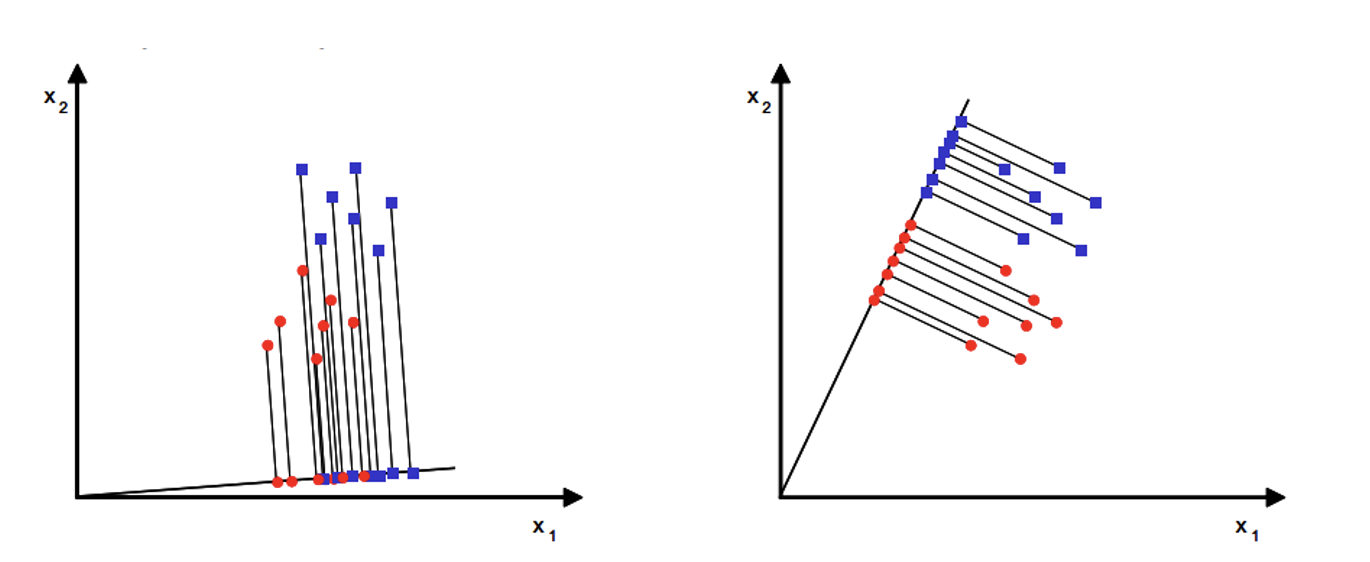
\includegraphics{./assets/projection.png}
\caption{Chiếu tập dữ liệu lên các đường thẳng khác nhau thì khả năng
phân biệt giữa các lớp cũng khác nhau.}
\end{figure}

Ta thấy phép chiếu bên trái đã có sự tối đa hóa về việc phân chia dữ
liệu độc lập nhau. Để có thể tìm được một vector chiếu tốt nhất, ta cần
xác định một quy tắc (rule) để phân chia dữ liệu.

Như đã phân tích trong Mục \href{}{2}, hai lớp được xem là phân biệt tốt
(discriminative) nếu khoảng cách giữa chúng lớn, tức là phương sai giữa
lớp (between-class variance) lớn, và dữ liệu trong từng lớp có mức độ
đồng nhất cao, tức là phương sai trong lớp (within-class variance) nhỏ.

Từ đó, phương pháp Linear Discriminant Analysis (LDA) có thể được hiểu
là một thuật toán nhằm tìm một phép chiếu tối ưu sao cho tỷ lệ giữa
phương sai giữa lớp và phương sai trong lớp đạt giá trị lớn nhất. Mục
tiêu của phương pháp này là tối ưu hóa khả năng phân biệt giữa các lớp
trong không gian đặc trưng.

Để cực đại hóa tỷ lệ giữa phương sai giữa lớp và phương sai trong lớp,
cần xác định một hàm mục tiêu phù hợp. Hàm mục tiêu này được xây dựng
dựa trên việc tìm cực trị của tỷ số giữa phương sai giữa lớp và phương
sai trong lớp nhằm mô hình hóa và tối ưu hóa quá trình phân tách giữa
các lớp.

\subsubsection{Xây dựng hàm mục
tiêu}\label{xuxe2y-dux1ef1ng-huxe0m-mux1ee5c-tiuxeau}

\begin{enumerate}
\def\labelenumi{\arabic{enumi}.}
\item
  \textbf{Phương sai giữa lớp (Between-Class Variance)}

  Gọi \(\mu_i\) là vector trung bình của các mẫu thuộc lớp
  \(\mathbf{C}_i\) trong không gian ban đầu \(\mathbb{R}^d\), được tính
  bằng:

  \[\mu_i = \frac{1}{N_i} \sum_{x_n \in \mathbf{C}_i} \mathbf{x}_n, \quad i = 1,2\]

  trong đó:

  \begin{itemize}
  \tightlist
  \item
    \(N_i\) là số lượng điểm dữ liệu thuộc lớp \(\mathbf{C}_i\).
  \item
    \(\mathbf{x}_n\) là một điểm dữ liệu thuộc lớp \(\mathbf{C}_i\).
  \item
    \(\boldsymbol{\mu}_i\) là vector trung bình của lớp \(\mathbf{C}_i\)
    trong không gian đặc trưng \(\mathbb{R}^d\).
  \end{itemize}

  Sau khi dữ liệu được chiếu lên phương \(\mathbf{w}\), trung bình mẫu
  trong không gian mới (không gian 1 chiều) được ký hiệu là \(m_i\):
  \[m_i = \frac{1}{N_i} \sum_{x_n \in \mathbf{C}_i} y_n\] Thay
  \(y_n = \mathbf{w}^T \mathbf{x}_n\), ta có:
  \[m_i = \frac{1}{N_i} \sum_{x_n \in \mathbf{C}_i} \mathbf{w}^T \mathbf{x}_n\]
  Sử dụng tính chất tuyến tính của tích vô hướng:
  \[m_i = \mathbf{w}^T \left( \frac{1}{N_i} \sum_{x_n \in \mathbf{C}_i} \mathbf{x}_n \right) = \mathbf{w}^T \mu_i\]
  \[\implies (m_1 - m_2) = w^T\mu_1 - w^T\mu_2 = w^T(\mu_1-\mu_2)\]

  Xét đẳng thức:
  \[(a^T b)^2 = (a^T b)(a^T b) = a^T b b^T a \quad (3.1)\] với \(a, b\)
  là hai véc tơ cùng chiều bất kỳ.

  Khi đó, phương sai giữa lớp (between-class variance) là:
  \[(m_1 - m_2)^2 =[w^T(\mu_1-\mu_2)]^2= w^T(\mu_1-\mu_2)(\mu_1-\mu_2)^Tw\]
  (Áp dụng đẳng thức ma trận \href{}{3.1})

  Đặt \(S_B=(\mu_1-\mu_2)(\mu_1-\mu_2)^T\), khi đó phương sai giữa lớp
  trở thành: \[(m_1 - m_2)^2 = \mathbf{w}^TS_B\mathbf{w}\]
\item
  \textbf{Phương sai trong lớp (Within-Class Variance)}

  Phương sai trong lớp (within-class variance) được định nghĩa là tổng
  phương sai của hai lớp \(s_1^2 + s_2^2\).

  Các phương sai trong lớp (within-class variances) được định nghĩa là:

  \[
   \begin{aligned}
   s_k^2 & =\sum_{n \in \mathbf{C}_1}\left(y_n-m_k\right)^2, \quad k=1,2, \ldots \\
   & =\sum_{n \in \mathbf{C}_1}\left(\mathbf{w}^T \mathbf{x}-\mathbf{w}^T \mu_k\right)^2 \\
   & =\sum_{n \in \mathbf{C}_1}\left(\mathbf{w}^T(\mathbf{x}_n-\mu_k)\right)^2 \\
   \end{aligned}
   \]

  \begin{itemize}
  \tightlist
  \item
    \textbf{Lưu ý:} Các phương sai trong lớp ở đây không được tính theo
    cách trung bình như phương sai thông thường. Mức độ ảnh hưởng của
    mỗi phương sai trong lớp phụ thuộc vào số lượng điểm dữ liệu trong
    lớp đó. Lớp có nhiều điểm dữ liệu hơn sẽ đóng góp nhiều hơn vào tổng
    phương sai trong lớp. Do đó, thay vì lấy trung bình, ta giữ nguyên
    tổng phương sai trong lớp bằng cách nhân phương sai với số lượng
    điểm dữ liệu trong lớp. Ta có thể hiểu phương sai trong lớp thực
    chất là phương sai thông thường nhân với số lượng điểm dữ liệu trong
    lớp đó.
  \end{itemize}

  Vậy phương sai trong lớp khi đó:

  \[\begin{aligned}
   s_1^2+s_2^2 & =\sum_{k=1}^2\sum_{n \in \mathbf{C}_1}\left(y_n-m_k\right)^2, \quad k=1,2, \ldots \\
   & =\sum_{k=1}^2\sum_{n \in \mathbf{C}_1}\left(\mathbf{w}^T \mathbf{x}-\mathbf{w}^T \mu_k\right)^2 \\
   & =\sum_{k=1}^2\sum_{n \in \mathbf{C}_1}\left(\mathbf{w}^T(\mathbf{x}_n-\mu_k)\right)^2 \\
   \end{aligned}
   \] Áp dụng đẳng thức ma trận \href{}{3.1} \[\begin{aligned}
   s_1^2+s_2^2 
   & =\sum_{k=1}^2\sum_{n \in 
   \mathbf{C}_1}\left(\mathbf{w}^T(\mathbf{x}_n-\mu_k)(\mathbf{x}_n-\mu_k)^T\mathbf{w} \right) \\
   & =\mathbf{w}^T\sum_{k=1}^2\sum_{n \in \mathbf{C}_1}\left((\mathbf{x}_n-\mu_k)(\mathbf{x}_n-\mu_k)^T\right)\mathbf{w}  \\
   \end{aligned}\]

  Đặt
  \(S_w = \sum_{k=1}^2\sum_{n \in \mathbf{C}_1}(\mathbf{x}_n-\mu_k)(\mathbf{x}_n-\mu_k)^T\)
  thì phương sai trong lớp sẽ trở thành:
  \[s_1^2 + s_2^2 = \mathbf{w} ^TS_w\mathbf{w}\]
\item
  \textbf{Hàm mục tiêu }

  LDA là thuật toán đi tìm giá trị lớn nhất của hàm mục tiêu:
  \[J(\mathbf{w}) = \frac{(m_1 - m_2)^2}{s_1^2+s_2^2} \]

  Bây giờ, bài toán tối ưu cho LDA trở thành:
  \[J(\mathbf{w}) =\frac{\mathbf{w}^TS_B\mathbf{w}}{\mathbf{w} ^TS_w\mathbf{w}} \quad \text{và} \quad \mathbf{w} = argmax \frac{\mathbf{w}^TS_B\mathbf{w}}{\mathbf{w} ^TS_w\mathbf{w}}\]

  với:

  \begin{itemize}
  \tightlist
  \item
    \(S_B=(\mu_1-\mu_2)(\mu_1-\mu_2)^T\)
  \item
    \(S_w = \sum_{k=1}^2\sum_{n \in \mathbf{C}_1}(\mathbf{x}_n-\mu_k)(\mathbf{x}_n-\mu_k)^T\)
  \end{itemize}
\end{enumerate}

\subsubsection{Bài toán tối ưu
hoá}\label{buxe0i-touxe1n-tux1ed1i-ux1b0u-houxe1}

Để tìm giá trị lớn nhất của hàm mục tiêu, ta thực hiện đạo hàm \(J(w)\)
và cho kết quả bằng \(0\). \[
\begin{aligned}
&  \frac{\partial J(\mathbf{w})}{\partial \mathbf{w}}=\frac{\partial}{\partial \mathbf{w}}\left(\frac{\mathbf{w}^T S_B \mathbf{w}}{\mathbf{w}^T S_{\mathbf{w}} \mathbf{w}}\right)=0 \\
& \Leftrightarrow\left(\mathbf{w}^T S_{\mathbf{w}} \mathbf{w}\right) \frac{d}{d \mathbf{w}}\left(\mathbf{w}^T S_B \mathbf{w}\right)-\left(\mathbf{w}^T S_B \mathbf{w}\right) \frac{d}{d \mathbf{w}}\left(\mathbf{w}^T S_{\mathbf{w}} \mathbf{w}\right)=0 \\
& \Leftrightarrow\left(\mathbf{w}^T S_{\mathbf{w}} \mathbf{w}\right) 2 S_B \mathbf{w}-\left(\mathbf{w}^T S_B \mathbf{w}\right) 2 S_{\mathbf{w}} \mathbf{w}=0 \\
& \Leftrightarrow\left(\frac{\mathbf{w}^T S_{\mathbf{w}} \mathbf{w}}{\mathbf{w}^T S_{\mathbf{w}} \mathbf{w}}\right) S_B \mathbf{w}-\left(\frac{\mathbf{w}^T S_B \mathbf{w}}{\mathbf{w}^T S_{\mathbf{w}} \mathbf{w}}\right) S_{\mathbf{w}} \mathbf{w}=0 \\
& \Leftrightarrow S_B \mathbf{w}-J(\mathbf{w}) S_{\mathbf{w}} \mathbf{w}=0 \\
& \Leftrightarrow S_{\mathbf{w}}^{-1} S_B \mathbf{w}-J(\mathbf{w}) \mathbf{w}=0 \\
& \Leftrightarrow S_{\mathbf{w}}^{-1} S_B \mathbf{w}=J(\mathbf{w}) \mathbf{w} \quad (3.2)\\
\end{aligned}
\]

Vì \(J(\mathbf{w})\) là một số vô hướng, nên suy ra \(\mathbf{w}\) phải
là một vector riêng của ma trận \(\mathbf{S}_W^{-1} \mathbf{S}_B\) ứng
với một trị riêng nào đó.

Hơn nữa, giá trị của trị riêng này chính bằng \(J(\mathbf{w})\). Do đó,
để hàm mục tiêu đạt giá trị lớn nhất, ta cần chọn trị riêng lớn nhất của
\(\mathbf{S}_W^{-1} \mathbf{S}_B\). Điều này có nghĩa là \(\mathbf{w}\)
sẽ là vector riêng ứng với trị riêng lớn nhất của
\(\mathbf{S}_W^{-1} \mathbf{S}_B\).

Vì \(\mathbf{w}\) là nghiệm của
\(\mathbf{w} = \arg\max \frac{\mathbf{w}^T S_B \mathbf{w}}{\mathbf{w}^T S_w \mathbf{w}}\),
nên bất kỳ bội số \(k \mathbf{w}\) (với \(k \neq 0\)) cũng là nghiệm.
Điều này là do giá trị hàm mục tiêu chỉ phụ thuộc vào hướng của
\(\mathbf{w}\), không phụ thuộc vào độ lớn của nó. Do đó, mọi nghiệm
thuộc về một đường thẳng trong không gian, không phải là một điểm duy
nhất.

\textbf{Chứng minh:}

Giả sử \(\mathbf{w}^*\) là nghiệm tối ưu, tức là:
\[J(\mathbf{w^*}) =\frac{\mathbf{w^*}^T S_B \mathbf{w^*}}{\mathbf{w^*}^T S_W \mathbf{w^*}} = \max_{\mathbf{w}} \frac{\mathbf{w}^T S_B \mathbf{w}}{\mathbf{w}^T S_W \mathbf{w}}\]

Xét bội số \(k \mathbf{w}^*\) với \(k \neq 0\), ta có: \[
\begin{aligned}
J(k\mathbf{w^*}) =
\frac{(k\mathbf{w}^*)^T S_B (k\mathbf{w}^*)}{(k\mathbf{w}^*)^T S_W (k\mathbf{w}^*)}  
= \frac{k^2 (\mathbf{w}^*)^T S_B (\mathbf{w}^*)}{k^2 (\mathbf{w}^*)^T S_W (\mathbf{w}^*)} 
= \frac{(\mathbf{w}^*)^T S_B (\mathbf{w}^*)}{(\mathbf{w}^*)^T S_W (\mathbf{w}^*)} = J(\mathbf{w})
\end{aligned} \quad (3.3)
\]

Ở đây ta thấy, khi giải bài toán LDA, hàm mục tiêu \(J(\mathbf{w})\) chỉ
phụ thuộc vào hướng của \(\mathbf{w}\) chứ không phụ thuộc vào độ lớn
của nó. Điều này có nghĩa là nếu \(\mathbf{w}\) là nghiệm, thì mọi bội
số \(k\mathbf{w}\) (với \(k \neq 0\)) cũng là nghiệm.

Để ``đóng băng'' độ lớn của \(\mathbf{w}\) hay chuẩn hóa độ lớn của nó
mà không làm thay đổi hướng, ta có thể đặt thêm điều kiện:
\[(\boldsymbol{\mu}_1 - \boldsymbol{\mu}_2)^T \mathbf{w} = J(\mathbf{w}) = L \quad (3.4)\]

với \(L\) là trị riêng lớn nhất của \(\mathbf{S}_W^{-1}\mathbf{S}_B\).

Điều này đảm bảo rằng khoảng cách giữa trung bình các lớp sau khi chiếu
(tính bằng
\(m_1 - m_2 = (\boldsymbol{\mu}_1 - \boldsymbol{\mu}_2)^T \mathbf{w}\))
đạt đúng mức tối ưu (tương đương với giá trị riêng lớn nhất \(L\)). Qua
đó, ta có được một hướng \(\mathbf{w}\) đã được chuẩn hóa phù hợp với
mục tiêu phân biệt tối ưu.

Bây giờ, chúng ta đi giải bài toán trị riêng \((3.2)\) với điều kiện
\((3.4)\).

Với
\(\mathbf{S}_B = (\boldsymbol{\mu}_1 - \boldsymbol{\mu}_2)(\boldsymbol{\mu}_1 - \boldsymbol{\mu}_2)^T\),
thay vào \((*)\):
\[L\mathbf{w}= J(\mathbf{w} ) \mathbf{w} =\mathbf{S}_W^{-1} \bigl[(\boldsymbol{\mu}_1 - \boldsymbol{\mu}_2)(\boldsymbol{\mu}_1 - \boldsymbol{\mu}_2)^T \bigr] \mathbf{w}  = \mathbf{S}_W^{-1} (\boldsymbol{\mu}_1 - \boldsymbol{\mu}_2)(\boldsymbol{\mu}_1 - \boldsymbol{\mu}_2)^T \mathbf{w}\]
mà \(L =(\boldsymbol{\mu}_1 - \boldsymbol{\mu}_2)^T \mathbf{w}\) nên:

\[
\begin{aligned}
&L \mathbf{w} = \mathbf{S}_W^{-1} (\boldsymbol{\mu}_1 - \boldsymbol{\mu}_2)(\boldsymbol{\mu}_1 - \boldsymbol{\mu}_2)^T \mathbf{w} \\
\Leftrightarrow \quad & L \mathbf{w} = L \mathbf{S}_W^{-1} (\boldsymbol{\mu}_1 - \boldsymbol{\mu}_2) \\
\Leftrightarrow \quad & \mathbf{w} = \mathbf{S}_W^{-1} (\boldsymbol{\mu}_1 - \boldsymbol{\mu}_2)
\end{aligned}
\]

Do \(\mathbf{w}\) là nghiệm, nên bất kỳ bội số \(k \mathbf{w}\) (với
\(k \neq 0\)) cũng là nghiệm (kết quả chứng minh \href{}{3.3}), nên
nghiệm tổng quát của \(\mathbf{w}\) là:
\[\mathbf{w} = \alpha\mathbf{S}_W^{-1} (\boldsymbol{\mu}_1 - \boldsymbol{\mu}_2), \quad \text{ với } \alpha \not = 0 \text{ bất kỳ}\]

\pagebreak

\subsubsection{Phương pháp phân
lớp}\label{phux1b0ux1a1ng-phuxe1p-phuxe2n-lux1edbp}

\pagebreak

\subsection{LDA với đa lớp}\label{lda-vux1edbi-ux111a-lux1edbp}

\section{Cài đặt và thực
nghiệm}\label{cuxe0i-ux111ux1eb7t-vuxe0-thux1ef1c-nghiux1ec7m}

\section{Kết luận và hướng phát
triển}\label{kux1ebft-luux1eadn-vuxe0-hux1b0ux1edbng-phuxe1t-triux1ec3n}

\section{Tham khảo}\label{tham-khux1ea3o}

\end{document}
